\documentclass[aspectratio=169]{beamer}
\usepackage[utf8]{inputenc}
\usepackage{amsmath,amssymb}
\usepackage[ngerman]{babel}
\usepackage{datetime}
\showdowfalse
\usepackage{array}
\usepackage{tabularx}
% use Swiss-style quotation marks (like in French)
\usepackage[autostyle,german=swiss]{csquotes}
\usepackage{framed} % or, "mdframed"
\makeatletter
\let\th@plain\relax
\makeatother
\usepackage[framed]{ntheorem}
\theoremstyle{plain}
\newframedtheorem{framed-def}{Definition}

\definecolor{FHNWyellow}{RGB}{253,231,14}
\definecolor{titlegrey}{RGB}{158,158,158}
\definecolor{bodygrey}{RGB}{188,188,188}
\definecolor{pitchblack}{rgb}{0, 0, 0}
\setbeamercolor{frametitle}{bg=FHNWyellow, fg=pitchblack}
\setbeamercolor{headline}{bg=FHNWyellow, fg=pitchblack}
\setbeamercolor{titlelike}{fg=pitchblack}
\setbeamercolor{title}{fg=pitchblack}
\setbeamercolor{item}{fg=pitchblack}
\setbeamercolor{section in toc}{fg=pitchblack}
\setbeamercolor{block body example}{fg=pitchblack,bg=bodygrey}
\setbeamercolor{block title example}{fg=pitchblack,bg=titlegrey}
\setbeamertemplate{section in toc}[sections numbered]
\usetheme{default}
\usecolortheme{wolverine}

\usepackage{tikz}
\usetikzlibrary{arrows.meta}
\usetikzlibrary{decorations.text}
\usetikzlibrary{shapes}
\usetikzlibrary{fit}
\usetikzlibrary{positioning, calc}
\usetikzlibrary{intersections}
\usepackage{./include/tikz-uml}
\tikzumlset{fill class=white}

\usepackage[export]{adjustbox}
\usepackage{changepage}

\makeatletter

\usepackage{listings}
\usepackage{listingsutf8}
\usepackage{courier}
\usepackage{graphicx}
\usepackage{textcomp}
\lstset{inputencoding=utf8/latin1}
\lstset{basicstyle=\tiny\ttfamily,breaklines=true}

\title[wodss]{Google Docs Light}
\subtitle{Midterm Presentation WODSS}
\author[Philip Colombo, Oliver Fabel, Melvin Johner, David Roth]{Philip Colombo\\Oliver Fabel\\Melvin Johner\\David Roth}
\newdate{date}{11}{04}{2022}
\date{\displaydate{date}}
\institute[FHNW]{
  Hochschule für Technik\\
  Fachhochschule Nordwestschweiz
}

\def\tabularxcolumn#1{m{#1}}
\beamertemplatenavigationsymbolsempty
\setbeamertemplate{footline}{
  \begin{tabularx}{\textwidth}{XX}
    \insertframenumber\hfill &
    \hfill\includegraphics[height=0.5cm]{media/fhnw_10mm.jpg}
  \end{tabularx}
}

\begin{document}

\lstdefinestyle{inlinefontsize}{
  basicstyle=\ttfamily\lst@ifdisplaystyle\scriptsize\fi
}
\lstset{style=inlinefontsize}

\begin{frame}
    \titlepage
    \thispagestyle{empty}
\end{frame}

\begin{frame}
    \frametitle{Inhaltsverzeichnis}
    \tableofcontents
\end{frame}

\section{Architektur}
\begin{frame}
    \frametitle{Architektur}
    \begin{minipage}{0.48\textwidth}
        \begin{itemize}
            \item Programmiersprache: TypeScript
            \item Store Framework: YJS
            \item Frontend Technologie: Vue.js
            \item Backend: Node.js
            \item Datenbank: MongoDB
            \item Middleware: Mosquitto
            \item Protokolle: Websockets und MQTT
        \end{itemize}
    \end{minipage}%
    \hfill
    \begin{minipage}{0.45\textwidth}
        \begin{figure}
            \centering
            \includegraphics[height=6cm]{media/wodss_architecture.png}
        \end{figure}
    \end{minipage}%
\end{frame}


\section{State Management}
\begin{frame}
    \frametitle{State Management}
    \begin{itemize}
        \item Jede Frontend Instanz des Editors inklusive des Backends führen den aktuellen Application State in einem eigenen Store.
        \item Dieser Store hält den Application State in zwei Instanzen der YJS Datenstruktur:
        \begin{description}
            \item[SyncedState] Wird im FE gerendert und im BE persistiert.
            \item[ShadowState] Wird mittels Aktionen(Messages / User Actions) manipuliert und dient zum Erstellen eines Diffs zum SyncedState.
        \end{itemize}
        \item Der Store bietet zwei Patch Methoden:
        \begin{description}
            \item[patchAsync] Aktualisiert beide States sofort und generiert periodisch Messages mit einem Patch.
            \item[patchSync] Aktualisiert im ersten Schritt den ShadowState, verschickt eine Message mit dem Patch und aktualisiert den SyncedState wenn der Patch verteilt wurde.
        \end{itemize}
        \item Aktionen die Konflikte generieren können, verwenden immer patchSync.
        \item Aktionen die möglichst rasch im FE angezeigt werden müssen und keine Konflikte generieren verwenden patchAsync.
    \end{itemize}
\end{frame}

\begin{frame}
    \frametitle{Store}
    \begin{itemize}
        \item Der Store verteilt jede State-Anpassung, je nach Änderung, sofort oder mit einem kleinen Delay über die Message Queue.
        \item Für alle Änderungen wird ein Diff erstellt und nur das Diff des States wird über die Message Queue verteilt.
        \item Beim Generieren dieser Diffs kommt YJS ins Spiel:
        \begin{itemize}
            \item YJS kann aus seiner Datenstruktur Patches generieren, welche kommutativ und idempotent angewendet werden können.
            \item Sollten Messages nicht in der korrekten Reihenfolge oder mehrfach ankommen haben alle Clients nach dem verteilen der Messages denselben Zustand.
            \item Die Message Queue garantiert eine excatly-once (QoS 2) Auslieferung aller Messages.
        \end{itemize}
    \end{itemize}
\end{frame}

\begin{frame}
    \frametitle{Patch Sync}
    So läuft ein synchrones Patch ab:
    \centering
    \includegraphics[height=6cm]{media/patchSync}\label{fig:Patch Sync Skizze}
\end{frame}

\begin{frame}
    \frametitle{Patch Async}
    So läuft ein asynchrones Patch ab:
    \centering
    \includegraphics[height=6cm]{media/patchAsync}\label{fig:Patch Async Skizze}
\end{frame}

\begin{frame}
    \frametitle{Inhalt des Stores}
    Der Shared State wird in folgendem Format in der YJS Datenstruktur gespeichert:
    \lstinputlisting[language=json, basicstyle=\tiny]{media/sharedStore.json}
\end{frame}





\section{YJS Dokument Internals}
\begin{frame}
    \frametitle{YJS Dokument Internals}
    \begin{itemize}
        \item Ein YJS\footnote[frame]{\tiny \url {https://github.com/yjs/yjs}} Dokument ist eine Implementierung des CRDT\footnote[frame]{\tiny \url{https://www.researchgate.net/publication/310212186_Near_Real-Time_Peer-to-Peer_Shared_Editing_on_Extensible_Data_Types}} Algorithmus, dass die interne Datenstruktur als \textit{shared types} zur Verfügung stellt.
        \item CRDT steht für \textit{Conflict-free replicated data types} und ist eine etwas neuere alternative zu \textit{OT operational transformation}.
        \item YJS nutzt CRDT um bei Datenmanipulationen die jeweiligen Differenzen zu berechnen und dieser wieder auf andere Stores anzuwenden.
        \item Dabei verwendet YJS \textit{State-based replication} und \textit{Version vectors} um die States in den verschiedenen Clients korrekt zu synchronisieren.
    \end{itemize}
    \centering
    \includegraphics[height=3cm]{media/crdt}\label{fig:CRDT Sample}
\end{frame}


\section{Backend und Persistenz}
\begin{frame}
    \frametitle{Backend und Persistenz}
    \begin{itemize}
        \item In unserem Konzept wird das Dokument nur von Clients bearbeitet.
        \item Das Backend hat nur die Aufgabe den State des Dokuments zu speichern und neuen Clients zur Verfügung zu stellen.
        \item Es hört - wie alle Clients - auf der Message Queue mit und schreibt alle State Änderungen in eine MongoDB.
    \end{itemize}
    \centering
    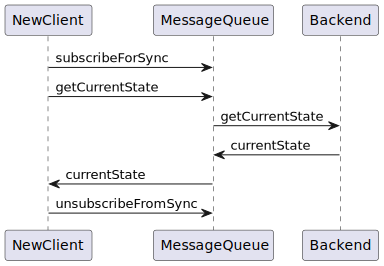
\includegraphics[height=5cm]{media/getStateFromBackend}\label{fig:Get State from Backend Diagramm}
\end{frame}


\section{MQTT Topics}
\begin{frame}
    \frametitle{MQTT Topics}
    \begin{itemize}
        \item Clients können sich auf der MOM auf einem Topic subscriben.
        \item Sie können in diesem Topic Messages absetzten und alle, die sich darauf registriert haben, erhalten die Message.
        \item Aktuell führen wir zwei Topics:
        \begin{description}
            \item[SyncTopic] Hier ist das Backend registriert und wartet auf sync Anfragen von Clients.
            Clients kommen nur kurz vorbei, um sich den aktuellen State zu abzufragen.
            \item[PatchTopic] Hier werden alle State Änderungen in Form von YJS Patches verteilt.
            Alle Clients + Backend sind hier registriert, wo sie ihre State Patches publizieren und fremde Patches empfangen.
        \end{itemize}
        \item Theoretisch wäre es möglich verschiedene Dokument Instanzen über verschiedene Topics zu verwalten.
    \end{itemize}
\end{frame}


\section{Ausblick}
\begin{frame}
    \frametitle{Work-in-Progress und Ausblick}
    \begin{itemize}
        \item Derzeit in Entwicklung:
        \begin{itemize}
            \item Implementation einer verteilten Mutex im \textit{Synchronized Store}.
            \item Refactoring der Session Verwaltung.
            \item \textit{Synchronized Store} vereinfachen: Konsolidieren von shadow und synchronized State.
        \end{itemize}
        \item Noch anstehende Arbeiten:
        \begin{itemize}
            \item Ein schönes UI implementieren.
            \item Persistenz Schicht im Backend umsetzen (derzeit nur In-Memory).
            \item Protokoll optimieren, evtl. QoS 1 für manche Nachrichten.
            \item Umfangreiche Performance Tests durchführen.
            \item Den Server mit HTTPS absichern.
            \item Logs im Backend einrichten.
            \item Evtl. authentifizierte Datenstruktur für den Store verwenden.
        \end{itemize}
    \end{itemize}
\end{frame}

\section{Demo}
\begin{frame}
    \frametitle{Demo}
    \begin{center}
        \begin{figure}
            
\includegraphics[height=6cm]{media/qr-wodss-sufa-li.eps}
        \end{figure}
        \url{http://wodss.sufa.li/\#Q2t4wmbnFf0x0wUhfY6XWb11dbBI2S}\\
        \href{http://wodss.sufa.li/fuzzy.html\#Q2t4wmbnFf0x0wUhfY6XWb11dbBI2S}{Fuzzy Test}
    \end{center}
\end{frame}

\title{Vielen Dank für die Aufmerksamkeit}
\subtitle{Fragen?}
\author{}
\institute{}
\date{}
\begin{frame}
    \maketitle
    \thispagestyle{empty}
\end{frame}

\end{document}
